%%%
% Plantilla de Presentación
% Modificación de una plantilla de Latex de LaTeXTemplates para adaptarla 
% al castellano y a las necesidades de escribir informática y matemáticas.
%
% Editada por: Mario Román
%
% License:
% CC BY-NC-SA 3.0 (http://creativecommons.org/licenses/by-nc-sa/3.0/)
%%%

%%%%%%%%%%%%%%%%%%%%%%%%%%%%%%%%%%%%%%%%%
% Beamer Presentation
% LaTeX Template
% Version 1.0 (10/11/12)
%
% This template has been downloaded from:
% http://www.LaTeXTemplates.com
%
% License:
% CC BY-NC-SA 3.0 (http://creativecommons.org/licenses/by-nc-sa/3.0/)
%
%%%%%%%%%%%%%%%%%%%%%%%%%%%%%%%%%%%%%%%%%

%----------------------------------------------------------------------------------------
%	PAQUETES Y CONFIGURACIÓN DEL DOCUMENTO
%----------------------------------------------------------------------------------------

\documentclass{beamer}

%% Configuración de la presentación
\mode<presentation> {
  %%% Selección de estilo
  % The Beamer class comes with a number of default slide themes
  % which change the colors and layouts of slides. Below this is a list
  % of all the themes, uncomment each in turn to see what they look like.

  %\usetheme{default}
  %\usetheme{AnnArbor}
  %\usetheme{Antibes}
  %\usetheme{Bergen}
  %\usetheme{Berkeley}
  %\usetheme{Berlin}
  %\usetheme{Boadilla}
  %\usetheme{CambridgeUS}
  %\usetheme{Copenhagen}
  %\usetheme{Darmstadt}
  %\usetheme{Dresden}
  %\usetheme{Frankfurt}
  %\usetheme{Goettingen}
  %\usetheme{Hannover}
  %\usetheme{Ilmenau}
  %\usetheme{JuanLesPins}
  %\usetheme{Luebeck}
  \usetheme{Madrid}
  %\usetheme{Malmoe}
  %\usetheme{Marburg}
  %\usetheme{Montpellier}
  %\usetheme{PaloAlto}
  %\usetheme{Pittsburgh}
  %\usetheme{Rochester}
  %\usetheme{Singapore}
  %\usetheme{Szeged}
  %\usetheme{Warsaw}

  %% Selección de color
  % As well as themes, the Beamer class has a number of color themes
  % for any slide theme. Uncomment each of these in turn to see how it
  % changes the colors of your current slide theme.

  %\usecolortheme{albatross}
  %\usecolortheme{beaver}
  %\usecolortheme{beetle}
  %\usecolortheme{crane}
  %\usecolortheme{dolphin}
  %\usecolortheme{dove}
  %\usecolortheme{fly}
  %\usecolortheme{lily}
  %\usecolortheme{orchid}
  %\usecolortheme{rose}
  %\usecolortheme{seagull}
  %\usecolortheme{seahorse}
  %\usecolortheme{whale}
  %\usecolortheme{wolverine}

  %% Configuración del pie de línea
  %\setbeamertemplate{footline} % To remove the footer line in all slides uncomment this line
  %\setbeamertemplate{footline}[page number] % To replace the footer line in all slides with a simple slide count uncomment this line
  %\setbeamertemplate{navigation symbols}{} % To remove the navigation symbols from the bottom of all slides uncomment this line
}

%% Fuentes de tamaño arbitrario
\usepackage{lmodern}

%% Gráficos
\usepackage{graphicx} % Allows including images
\usepackage{booktabs} % Allows the use of \toprule, \midrule and \bottomrule in tables
\usepackage{wrapfig}

%% Algoritmos
\usepackage{algorithm}
\usepackage{algorithmic}
\floatname{algorithm}{Algoritmo}
\renewcommand{\listalgorithmname}{Lista de algoritmos}
\renewcommand{\algorithmicrequire}{\textbf{Entrada:}}
\renewcommand{\algorithmicensure}{\textbf{Salida:}}
\renewcommand{\algorithmicend}{\textbf{Fin}}
\renewcommand{\algorithmicif}{\textbf{Si}}
\renewcommand{\algorithmicthen}{\textbf{Entonces}}
\renewcommand{\algorithmicelse}{\textbf{En otro caso}}
\renewcommand{\algorithmicelsif}{\algorithmicelse,\ \algorithmicif}
\renewcommand{\algorithmicendif}{\algorithmicend\ \algorithmicif}
\renewcommand{\algorithmicfor}{\textbf{Para }}
\renewcommand{\algorithmicforall}{\textbf{Para cada}}
\renewcommand{\algorithmicdo}{\textbf{}}
\renewcommand{\algorithmicendfor}{\algorithmicend\ \algorithmicfor}
\renewcommand{\algorithmicwhile}{\textbf{Mientras}}
\renewcommand{\algorithmicendwhile}{\algorithmicend\ \algorithmicwhile}
\renewcommand{\algorithmicloop}{\textbf{Repetir}}
\renewcommand{\algorithmicendloop}{\algorithmicend\ \algorithmicloop}
\renewcommand{\algorithmicrepeat}{\textbf{Repetir}}
\renewcommand{\algorithmicuntil}{\textbf{Hasta que}}
\renewcommand{\algorithmicprint}{\textbf{Imprimir}} 
\renewcommand{\algorithmicreturn}{\textbf{Devolver}} 
\renewcommand{\algorithmictrue}{\textbf{Verdadero }} 
\renewcommand{\algorithmicfalse}{\textbf{Falso }} 
\renewcommand{\algorithmicand}{\textbf{Y}}
\renewcommand{\algorithmicor}{\textbf{O}}
\renewcommand{\algorithmicnot}{\textbf{No}}

%%% Castellano.
% noquoting: Permite uso de comillas no españolas.
% lcroman: Permite la enumeración con numerales romanos en minúscula.
% fontenc: Usa la fuente completa para que pueda copiarse correctamente del pdf.
\usepackage[spanish,es-noquoting,es-lcroman]{babel}
\usepackage[utf8]{inputenc}
\usepackage[T1]{fontenc}
\selectlanguage{spanish}

%----------------------------------------------------------------------------------------
%	TÍTULO
%----------------------------------------------------------------------------------------

\title[AES process]{Advanced Encryptation Standard process} % The short title appears at the bottom of every slide, the full title is only on the title page

\author[Óscar Bermúdez, P. García Sánchez]{
	Óscar Bermúdez Garrido\\	
	\href{http://www.github.com/oxcar103}{@oxcar103}\\
	Pedro Abelardo García Sánchez
} % Your name
\institute[UGR] % Your institution as it will appear on the bottom of every slide, may be shorthand to save space
{
  Universidad de Granada \\ % Your institution for the title page
  \medskip
  \textit{oscarbg@correo.ugr.es} % Your email address
}
\date{\today} % Date, can be changed to a custom date



\begin{document}

%% Diapositiva de título.
\begin{frame}
\titlepage % Print the title page as the first slide
\end{frame}

% Diapositiva de contenidos.
% Throughout your presentation, if you choose to use \section{} and \subsection{} commands, 
% these will automatically be printed on this slide as an overview of your presentation
\begin{frame}
  \frametitle{Contenidos} % Table of contents slide, comment this block out to remove it
  \tableofcontents
\end{frame}



%----------------------------------------------------------------------------------------
%	PRESENTACIÓN
%----------------------------------------------------------------------------------------

%------------------------------------------------
\section{Definiciones Generales} % Sections can be created in order to organize your presentation into discrete blocks, all sections and subsections are automatically printed in the table of contents as an overview of the talk
%------------------------------------------------

	\subsection{Conceptos básicos} % A subsection can be created just before a set of slides with a common theme to further break down your presentation into chunks
	\begin{frame}
	\frametitle{Conceptos básicos}
	\begin{itemize}
		\item \textbf{texto plano} o \textit{plaintext}

		\item \textbf{texto cifrado} o \textit{cyphertext}.
		
		\item \textbf{clave o llave principal}.
		
		\item \textbf{clave o llave de ronda}.
	\end{itemize}
	\end{frame}
	
	\subsection{Criptoanálisis}
	\begin{frame}
	\frametitle{Criptoanálisis}
	\begin{itemize}
		\item \textbf{Criptoanálisis}, búsqueda de huecos que nos permitan conocer el mensaje o la clave empleada.
	
		\uncover<2>{\item \textbf{Confusión}, cada bit del criptograma depende de varios bits de la clave.
		
		\item \textbf{Difusión}, cada cambio en un bit del mensaje altera la mitad de los bits del criptograma.}
		
		\item \textbf{Key whitening}, mezcla parte de la clave con el mensaje antes y después de cifrar el resultado. Eficaz frente al ataque \textit{meet-in-the-middle}.
	\end{itemize}
	\end{frame}

	\subsection{Redes de Feistel}
	\begin{frame}
	\frametitle{Redes de Feistel}
	\begin{wrapfigure}{r}{0.3\linewidth}
		\centering
		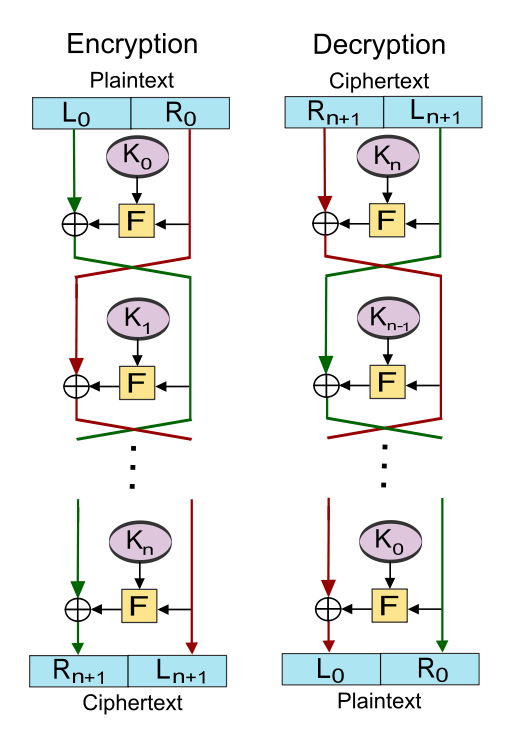
\includegraphics[height=5.5cm]{./Images/Feistel_cipher.png}\\
	\end{wrapfigure}

	Ejemplo de red de Feistel simple:

	\begin{algorithm}[H]
	\begin{algorithmic}[1]
		\REQUIRE \ \\
		\texttt{$L_0$}, mitad izquierda del plaintext\\
		\texttt{$R_0$}, mitad derecha del plaintext\\
		\FOR{\texttt{$i = 0 \rightarrow n$}}
		\STATE{\texttt{$L_{i+1} = R_i$}}
		\STATE{\texttt{$R_{i+1} = L_i \oplus F(R_i, K_i)$}}
		\ENDFOR
		
		\RETURN{\texttt{($R_{n+1}, L_{n+1}$)}}
	\end{algorithmic}
	\caption{Redes de Feistel.}
	\end{algorithm}
	
	\textbf{Función de Feistel}, combina el bloque y la clave de ronda, proporcionando confusión y difusión.

	Es \textbf{simétrico}, es decir, el mismo algoritmo cifra y descifra.
	\end{frame}

	\subsection{Redes de Sustitución-Permutación}
	\begin{frame}
	\frametitle{Redes de Sustitución-Permutación}
	\begin{wrapfigure}{r}{0.4\textwidth} %this figure will be at the right
		\centering
		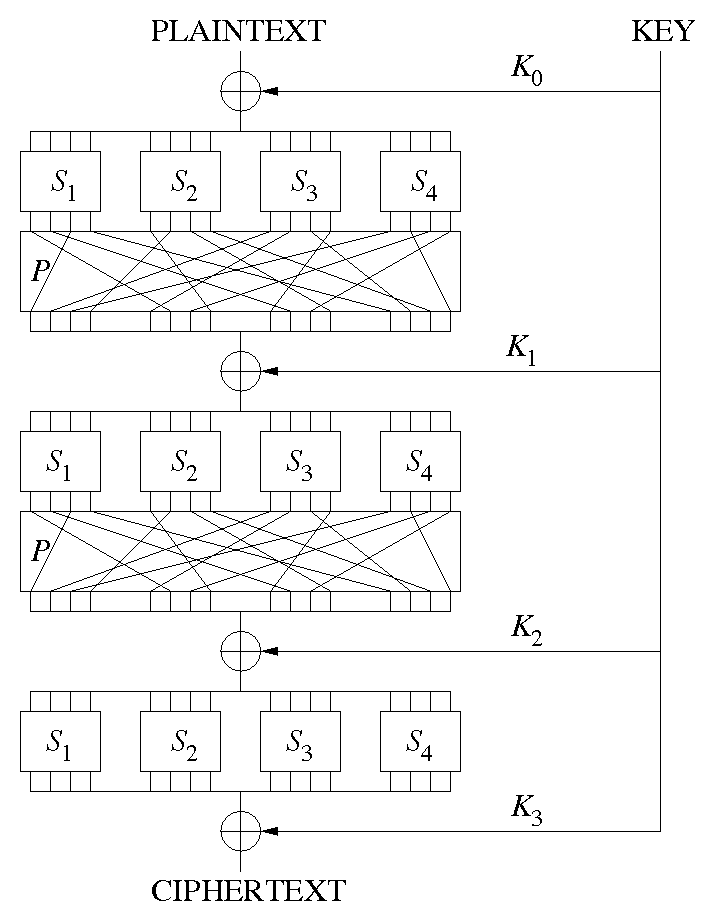
\includegraphics[height=0.4\textwidth]{./Images/SubstitutionPermutationNetwork.png}
	\end{wrapfigure}
	
	El núcleos de estas redes son las cajas de sustitución (\textit{S-box}) y permutación (\textit{P-box}):
	
	\begin{itemize}
		\item \textbf{S-box}, función biyectiva cumple la propiedad de difusión.
	
		\item \textbf{P-box}, conecta las \textit{S-boxes} de una capa con las \textit{S-boxes} de la siguiente.
	\end{itemize}
	
	Para el cifrado, se hacen pasar una o más veces por las \textit{S-box} y las \textit{P-box}.
	
	En el descifrado, se utilizan las inversas de las cajas.
	\end{frame}

	\subsection{Cuerpos finitos}
	\begin{frame}
	\frametitle{Cuerpos finitos: Definiciones}
	\begin{itemize}
		\item Llamaremos \textbf{cuerpo finito} o cuerpo de Galois al cuerpo definido sobre un conjunto finito de elementos.

		\item Sea $a \in F^*$, llamamos \textbf{orden} de $a$ al menor $d \in \mathbb{N}$ tal que $a^d = 1$.
		
		\item Dado un cuerpo $F$ finito de $n$ elementos, diremos que $g$ es un \textbf{generador} si su orden es $n-1$, es decir, sus potencias generan $F^*$.
	\end{itemize}
	\end{frame}

	\begin{frame}
	\frametitle{Cuerpos finitos: Resultados}
	\begin{itemize}
		\item El orden de todo elemento $a \in F^*$ divide a $n-1$.
		
		\item Todo cuerpo finito tiene un generador. De hecho, tiene $\varphi (n-1)$ generadores distintos.
		
		\item Si $F_q$ es un cuerpo con $q = p^f$ elementos, entonces todo elemento cumple la ecuación $X^q - X = 0$ y $F_q$ es precisamente el conjunto de raíces de esta ecuación.
		
		\item Para cada $q = p^f$, el polinomio $X^q - X$ se factoriza en $F_p[X]$ como el producto de todos los polinomios mónicos irreducibles de grado $d|f$.
		
		\item En la práctica, para construir $F_q$ con $q = p^f$, se toma un polinomio $f(X)$ irreducible de grado $f$ en $\mathbb{Z}_p[X]$ y se calcula $F_p[X] / \langle f(X) \rangle$.
		
		\item Todo cuerpo finito tiene $p^n$ elementos con $p$ primo y $n$ entero positivo.
	\end{itemize}
	\end{frame}


\section{Técnicas de Criptoanálisis}
	\begin{frame}
		\frametitle{Técnicas de Criptoanálisis}
		\begin{itemize}
			\item \textbf{Fuerza bruta}, probar de manera exhaustiva todas las posibles claves.
			
			\item \textbf{Criptoanálisis lineal}, intenta aproximar la acción del algoritmo a alguna transformación afín.
			
			\item \textbf{Criptoanálisis diferencial}, estudia cómo afectan las variaciones de la entrada a su salida.
			
			\item \textbf{Criptoanálisis diferencial-lineal}, combinación de ambas técnicas explicadas anteriormente.
		\end{itemize}
	\end{frame}
	
\section{Modos de operación}
	\begin{frame}
	\frametitle{Modos de operación}
		Los \textit{modos de operación} transforman el mensaje original en varios submensajes del tamaño adecuado.
		
		\begin{itemize}
			\item \textit{Electronic Codebook} (\textbf{ECB}).
			
			\item \textit{Cipher Block Chaining} (\textbf{CBC}).
			
			\item \textit{Output Feedback} (\textbf{OFB})
			
			\item \textit{Cipher Feedback} (\textbf{CFB}).
			
			\item \textit{Counter} (\textbf{CTR}).
		\end{itemize}
	\end{frame}
		
\section{AES process}
	\begin{frame}
	\frametitle{Un poco de historia del AES process}
	El estándar anterior (\textit{DES}) dejó de ser seguro por la longitud de su clave. Surgió la necesidad de un nuevo estándar.
	
	El Instituto Nacional de Estándares y Tecnología(\textit{NIST}) de los Estados Unidos proclamó en enero de 1997 el \textit{AES process}.
	
	Los criterio del concurso público fueron:
	\begin{itemize}
		\item Aceptar un tamaño de bloque de 128 bits.
		
		\item Aceptar un tamaño de clave de 128, 192 y 256 bits.
		
		\item Ser accesible públicamente.
		
		\item Ser de dominio público.
		
		\item Tener eficiencia tanto hardware como software.
	\end{itemize}
	\end{frame}
	
	\begin{frame}
	\frametitle{Finalistas del AES process}
	Muchos algoritmos se presentaron pero tras una conferencia en 1998 se destacaron cinco finalistas:
	\begin{wrapfigure}{r}{0.5\linewidth}
		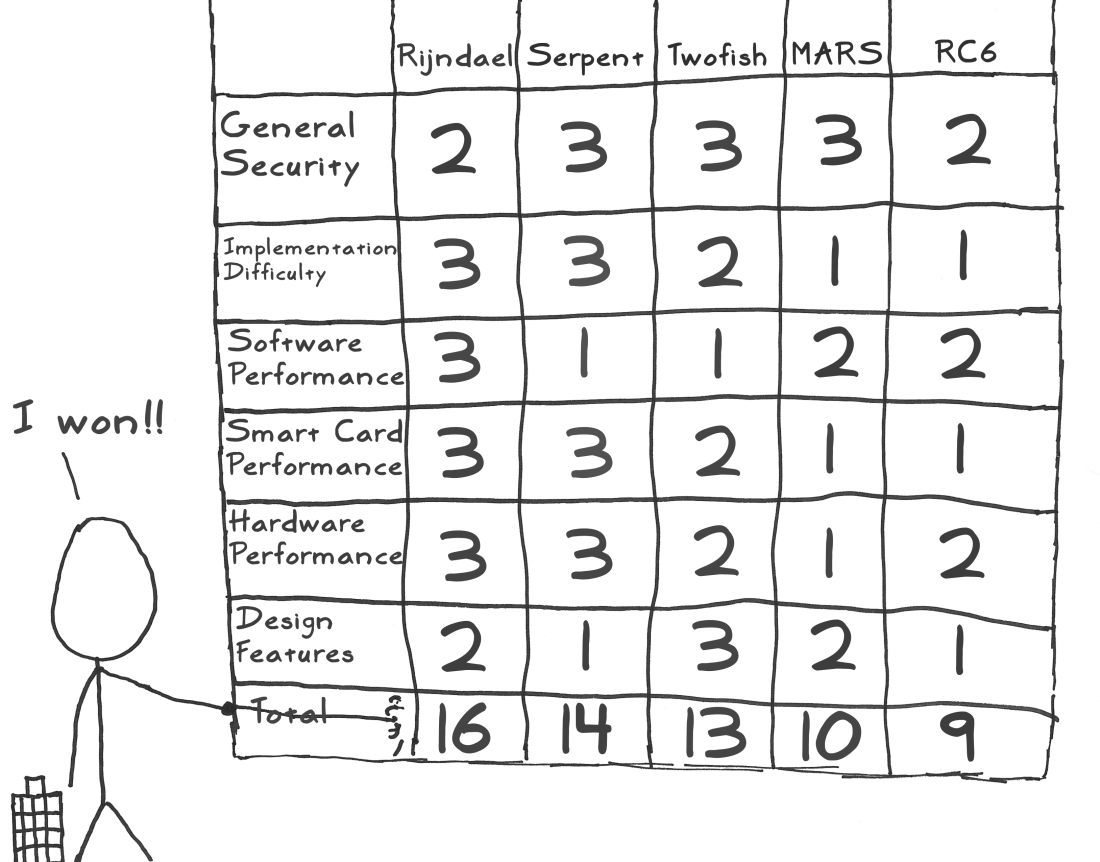
\includegraphics[width=0.85\linewidth]{./Images/xkcd-votos.png}\\
	\end{wrapfigure}
	\begin{itemize}
		\item \textit{MARS}
		\item \textit{RC6}
		\item \textit{Rijndael}
		\item \textit{Serpent}
		\item \textit{Twofish}
	\end{itemize}
	
	\vspace{1cm}
	
	En una segunda conferencia en 1999, se realizó una votación en la que \textit{Rijndael} se convirtió en \textbf{AES}.
	\end{frame}
	
	\subsection{Rijndael}
	\begin{frame}
	\frametitle{Rijndael - Presentación}
	\begin{itemize}
		\item \textit{Rijndael} fue desarrollado por Vincent Rijmen y Joan Daemen
		
		\item Basado en redes de sustitución-permutación y su resistencia está en los Cuerpos finitos de las $S-boxes$ y de \textit{MixColumns}.
		
		\item Eficiencia en sistemas con bajos recursos.
		
		\item Número de rondas dependiente del tamaño de clave: 10 para 128-bits, 12 para 192-bits y 14 para 256-bits.
		
		\item Las funciones \textit{MixColumns} y \textit{ShiftRows} son su fuente principal de difusión.
	\end{itemize}	
	\end{frame}

	\begin{frame}
	\frametitle{Rijndael - Algoritmo}
	El esqueleto principal de \textit{Rijndael} sería:
	\begin{algorithm}[H]
		\begin{algorithmic}[1]
			\REQUIRE \ \\
			\texttt{$P$}, plaintext\\
			
			\STATE{\texttt{$B = AddRoundKey(P, K_0)$}}
			\FOR{\texttt{$i = 1 \rightarrow n$}}
			\STATE{\texttt{$B = SubBytes(B)$},}
			\STATE{\texttt{$B = ShiftRows(B)$},}
			\IF{\texttt{$i \neq n$}}
			\STATE{\texttt{$B = MixColumns(B)$}, si no es la última ronda}
			\ENDIF
			\STATE{\texttt{$B = AddRoundKey(B, K_i)$},}
			\ENDFOR
			\RETURN{\texttt{$C = B$}}
		\end{algorithmic}
		\caption{Algoritmo de Rijndael presentado al AES.}
	\end{algorithm}
	\end{frame}
	
	\begin{frame}
	\frametitle{Rijndael - AddRoundKey}
		\Huge{\centerline{$AddRoundKey(A, B) = A \oplus B$.}}
		\Huge{\centerline{\only<2>{\alert{No hay más.}}}}
	\end{frame}

	\begin{frame}
	\frametitle{Rijndael - SubBytes}
	\begin{itemize}

		\item La función de \textit{SubBytes} es la $S-box$ de la red.
		
		\only<-2>{\item Convierte su entrada en el polinomio asociado del cuerpo $\textit{GF}(2^8) = \textit{GF}(2)[x]/(x^8+x^4+x^3+x+1)$
		
		\item Calcula entonces su inversa y lo devuelve a su representación binaria.
		
		\uncover<2>{\item Se utiliza una tabla con las inversas pre-calculadas para agilizar el proceso. Por convenio, el polinomio 0 es su propia inversa.}
		
		\item Por último, se hace pasar por la transformación afín:
		$$\begin{bmatrix}
		s_0 \\
		s_1 \\
		s_2 \\
		s_3 \\
		s_4 \\
		s_5 \\
		s_6 \\
		s_7 \\
		\end{bmatrix} =
		\begin{bmatrix}
		1 & 0 & 0 & 0 & 1 & 1 & 1 & 1 \\
		1 & 1 & 0 & 0 & 0 & 1 & 1 & 1 \\
		1 & 1 & 1 & 0 & 0 & 0 & 1 & 1 \\
		1 & 1 & 1 & 1 & 0 & 0 & 0 & 1 \\
		1 & 1 & 1 & 1 & 1 & 0 & 0 & 0 \\
		0 & 1 & 1 & 1 & 1 & 1 & 0 & 0 \\
		0 & 0 & 1 & 1 & 1 & 1 & 1 & 0 \\
		0 & 0 & 0 & 1 & 1 & 1 & 1 & 1 \\
		\end{bmatrix} \cdot
		\begin{bmatrix}
		b_0 \\
		b_1 \\
		b_2 \\
		b_3 \\
		b_4 \\
		b_5 \\
		b_6 \\
		b_7 \\
		\end{bmatrix} +
		\begin{bmatrix}
		1 \\
		1 \\
		0 \\
		0 \\
		0 \\
		1 \\
		1 \\
		0 \\
		\end{bmatrix}$$}
	\end{itemize}

	\only<3>{\begin{figure}
		\centering
		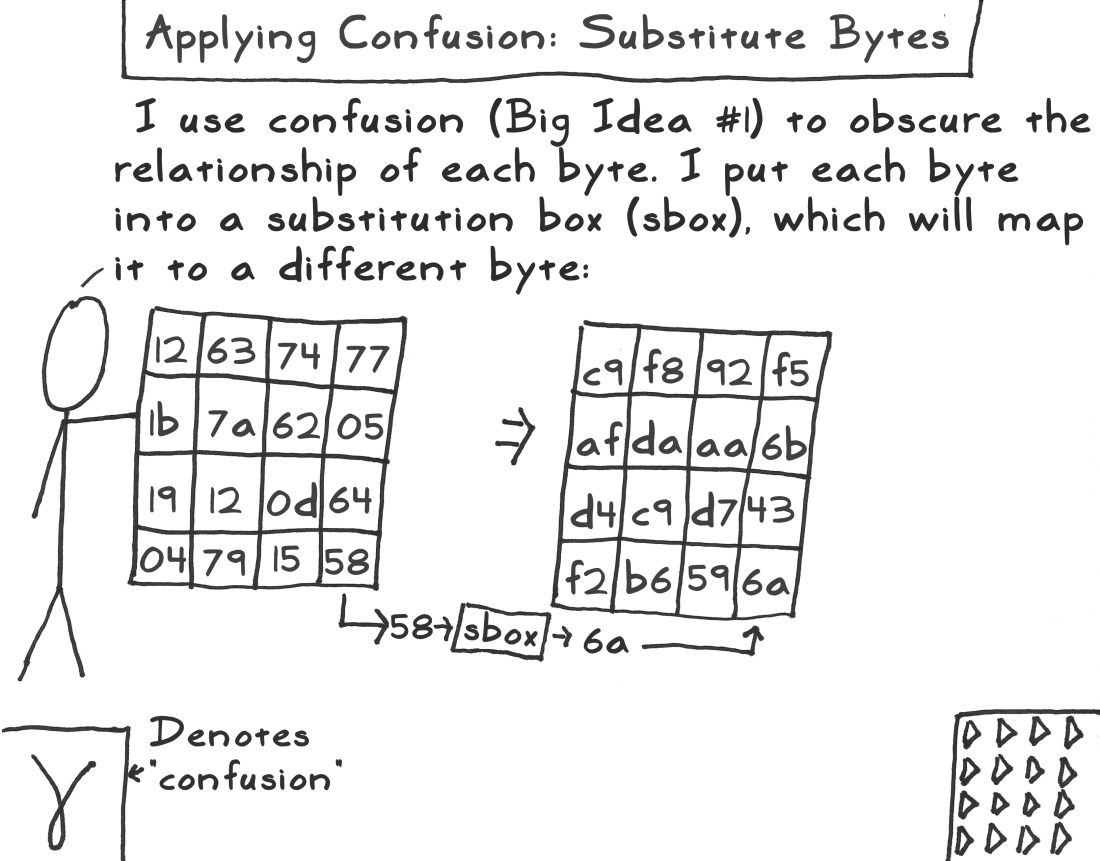
\includegraphics[width=0.75\linewidth]{./Images/xkcd-subbytes.png}
	\end{figure}}

	\end{frame}
	
	\begin{frame}
	\frametitle{Rijndael - ShiftRows}
	\begin{wrapfigure}{r}{0.55\linewidth}
		\centering
		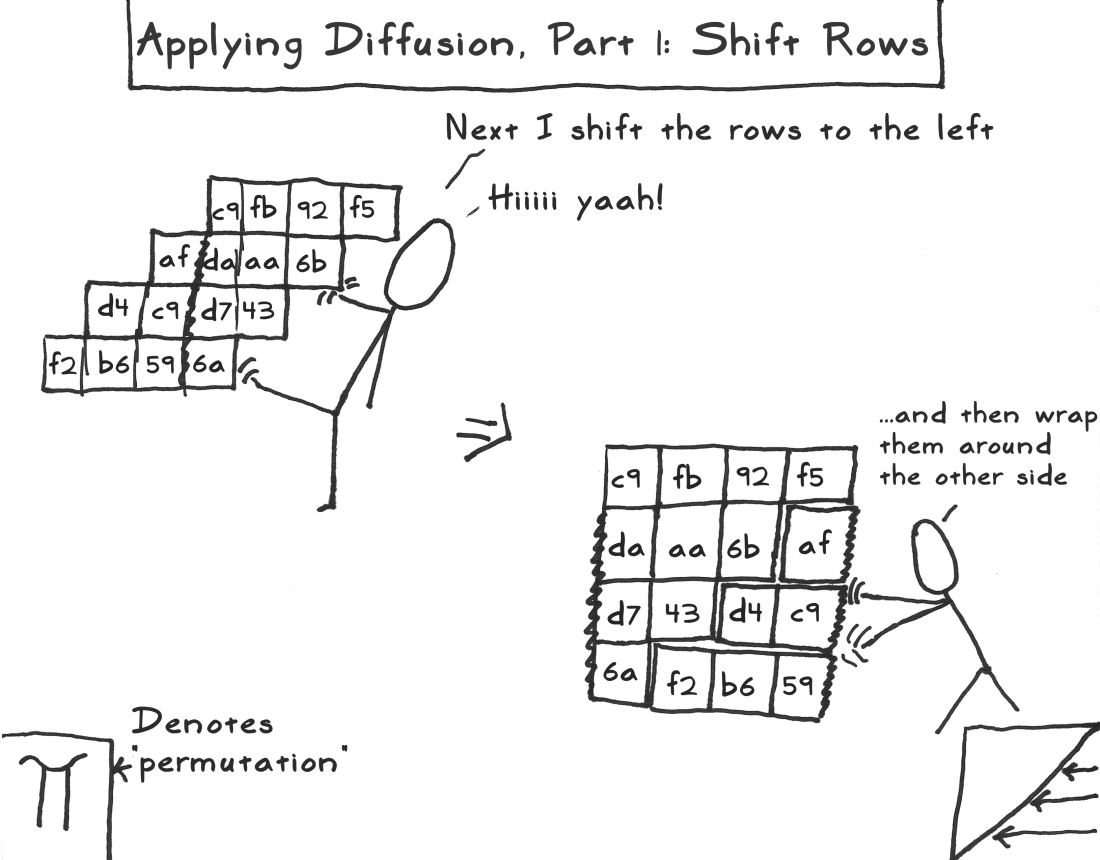
\includegraphics[height=4.5cm]{./Images/xkcd-shiftrows.png}
	\end{wrapfigure}

	\textit{ShiftRows} trata la entrada como una matriz y rota de distinta manera cada fila:
	
	\begin{algorithm}[H]
		\begin{algorithmic}[1]
			\REQUIRE \ \\
			\texttt{$R_0, R_1, R_2, R_3$}, Filas de la matriz\\
			\FOR{\texttt{$i \rightarrow 3$}}
			\STATE{\texttt{$R_i = R_i <<< i$}}
			\ENDFOR
		\end{algorithmic}
		\caption{Función ShiftRows.}
	\end{algorithm}	
	\end{frame}
	
	\begin{frame}
	\frametitle{Rijndael - MixColumns}
	\begin{itemize}
		\item \textit{MixColumns} convierte cada columna en un polinomio $p(x) = ax^3 + bx^2 + cx + d$ con $a, b, c, d \in \textit{GF}(2^8)$ los coeficientes de las columnas
	
		\item Multiplica el polinomio obtenido por un polinomio constante $q(x) = 3x^3 + x^2 + x + 2$ y se reduce módulo $x^4 + 1$
		
		\item Se devuelve el nuevo polinomio.
		
		\only<2>{\item En la práctica, se memoriza la matriz que realiza estos pasos y se aplica a cada columna:
		$$\begin{bmatrix}
		s_0 \\
		s_1 \\
		s_2 \\
		s_3 \\
		\end{bmatrix} =
		\begin{bmatrix}
		2 & 3 & 1 & 1 \\
		1 & 2 & 3 & 1 \\
		1 & 1 & 2 & 3 \\
		3 & 1 & 1 & 2 \\
		\end{bmatrix} \cdot
		\begin{bmatrix}
		b_0 \\
		b_1 \\
		b_2 \\
		b_3 \\
		\end{bmatrix}$$}
	\end{itemize}

	\only<1>{\begin{figure}
		\centering
		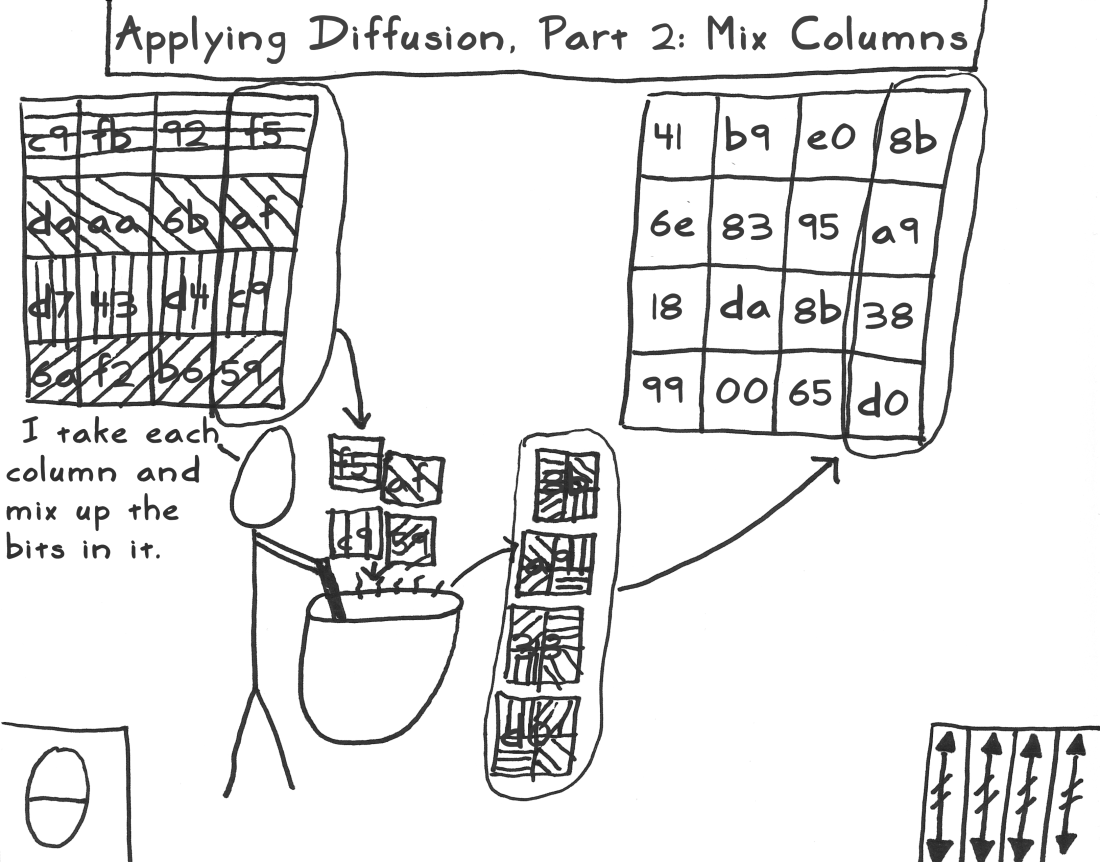
\includegraphics[width=0.5\linewidth]{./Images/xkcd-mixcolumns.png}
	\end{figure}}
	\end{frame}

	\begin{frame}
	\frametitle{Rijndael - Fácil, ¿no?}
	\begin{figure}
		\centering
		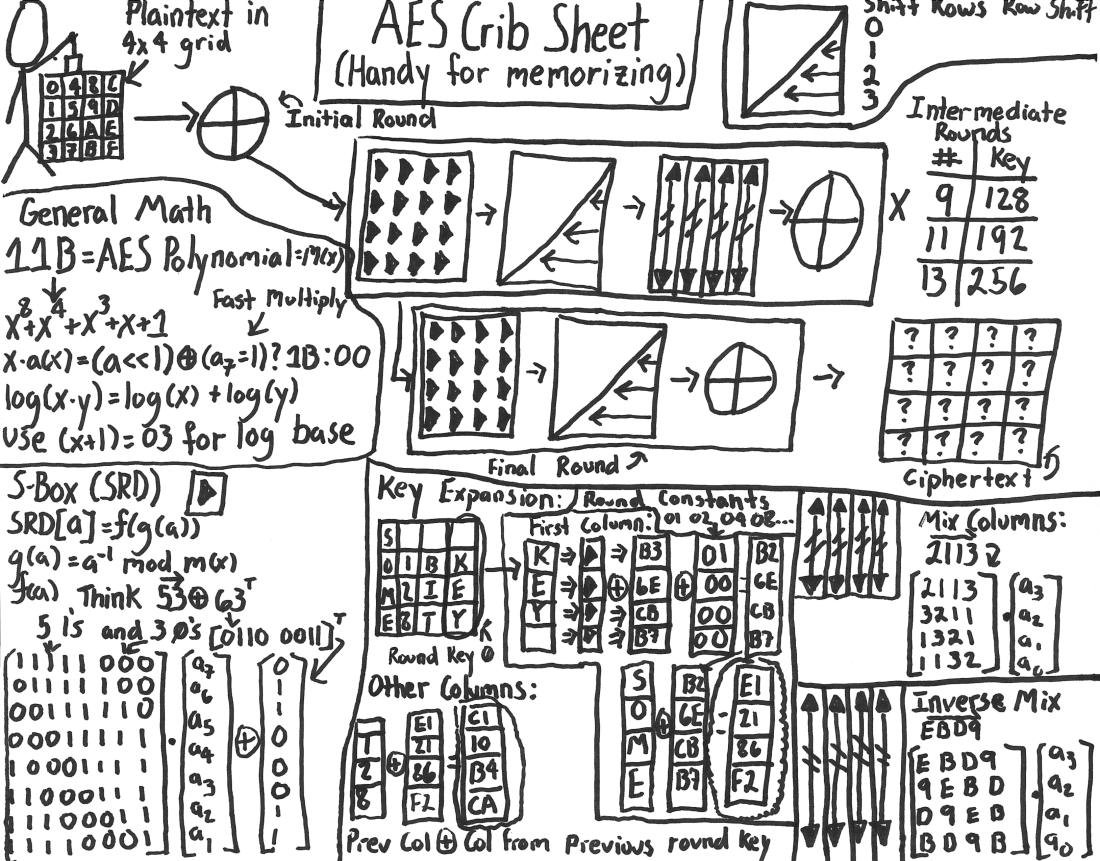
\includegraphics[width=0.8\linewidth]{./Images/xkcd-AES.png}
	\end{figure}
	\end{frame}
	
	\subsection{Serpent}
	\begin{frame}
	\frametitle{Serpent - Presentación}
	\begin{itemize}
		\item \textit{Serpent} fue creado por Ross Anderson, Eli Biham y Lars Knudsen.
		
		\item Fue diseñado para ejercutarse en paralelo.
			
		\item Sus desarrolladores buscaba un gran margen de seguridad.
		
		\item Recibió el menor número de votos negativos.
		
		\item Es una red de sustitución-permutación de 32 rondas con 8 $S-boxes$ diferentes y una aplicación lineal
		
		\item Las $S-boxes$ se obtienen a partir de variaciones de las que usaba \textit{DES}.
	\end{itemize}	
	\end{frame}
	
	\begin{frame}
	\frametitle{Serpent - Algoritmo}
	\begin{algorithm}[H]
		\begin{algorithmic}[1]
		\REQUIRE \ \\
		\texttt{$P$}, plaintext\\
		
		\STATE{\texttt{$B_0 = IP(P)$}, permutación inicial.}
		\FOR{\texttt{$i = 0 \rightarrow 31$}}
		\STATE{\texttt{$B' = S_{i \mod 8}[B_i \oplus K_i]$}}
		\IF{\texttt{$i \equiv 31$}}
		\STATE{\texttt{$B_{i+1} = B' \oplus K_{32}$}, última ronda.}
		\ELSE
		\STATE{\texttt{$B_{i+1} = L(B')$}, ronda normal.}
		\ENDIF
		\ENDFOR
		\STATE{\texttt{$C = FP(B_{32})$}, permutación final.}
		\RETURN{\texttt{$C$}}
		\end{algorithmic}
	\caption{Algoritmo de Serpent presentado al AES.}
	\end{algorithm}
	\end{frame}
	
	\subsection{MARS}
	\begin{frame}
	\frametitle{MARS - Presentación}
	\begin{itemize}
		\item \textit{MARS} fue desarrollado por \textit{IBM} de la mano de \textit{Don Coppersmith}, al igual que \textit{DES}.

		\item Es complejo y poco elegante. Introdujo valores sin justificar.

		\item \textit{MARS} está basado en redes de Feistel de tipo 3:
		\begin{algorithm}[H]
			\begin{algorithmic}[1]
				\REQUIRE \ \\
				\texttt{$A_0, B_0, C_0, D_0$}, plaintext dividido en 4 partes\\
				\FOR{\texttt{$i = 0 \rightarrow n$}}
				\STATE{\texttt{$D_{i+1} = A_i$}, esta parte pasa sin modificar.}
				\STATE{\texttt{$(F_1, F_2, F_3) = F(A_i, K_i)$}, dividimos la salida en 3 partes.}
				\STATE{\texttt{$C_{i+1} = D_i \oplus F_3 \qquad$} en el resto, se combinan}
				\STATE{\texttt{$B_{i+1} = C_i \oplus F_2 \qquad$} los valores antiguos con la}
				\STATE{\texttt{$A_{i+1} = B_i \oplus F_1 \qquad $} salida de la función de Feistel.}
				\ENDFOR
				
				\RETURN{\texttt{($A_{n+1}, B_{n+1}, C_{n+1}, D_{n+1}$)}}
			\end{algorithmic}
			\caption{Redes de Feistel de tipo 3.}
		\end{algorithm}
	\end{itemize}
	\end{frame}

	\begin{frame}
	\frametitle{MARS - Algoritmo}
	\textit{MARS} se puede dividir en 3 partes:
	\only<1>{\begin{algorithm}[H]
		\begin{algorithmic}[1]
			\REQUIRE \ \\
			\texttt{$A, B, C, D$}, plaintext dividido en 4 partes de 32 bits\\
			\texttt{$K$}, clave expandida compuesta de 40 partes de 32 bits\\
			
			\STATE{\texttt{$(A,B,C,D) = (A,B,C,D) + (K[0],K[1],K[2],K[3])$}, \textit{Key whitening}}
			\STATE{\texttt{Forward Mixing}}
			\STATE{\texttt{Cryptographic Core}}
			\STATE{\texttt{Backwards Mixing}}
			
			\STATE{\texttt{$(A,B,C,D) = (A,B,C,D) - (K[36],K[37],K[38],K[39])$}, \textit{Key whitening}}
			\RETURN{\texttt{($A, B, C, D$)}}
		\end{algorithmic}
		
		\caption{Algoritmo de MARS presentado al AES.}
	\end{algorithm}}

	\only<2>{\begin{itemize}
		\item \textit{Forward Mixing}, serie de transformaciones lineales que favorecen la difusión.
		\item \textit{Cryptographic Core}, se basa en la red de Feistel de tipo 3 mejorando tanto la confusión como la difusión.
		\item \textit{Backward Mixing}, invierte las transformaciones lineales desarrolladas en el \textit{Forward Mixing}. 
	\end{itemize}}
	\end{frame}

	\subsection{Twofish}
	\begin{frame}
	\frametitle{Twofish - Presentación}
	\begin{itemize}
		\item \textit{TwoFish} fue desarrollado por Bruce Schneider, John Kelsey y Niels Ferguson.
		
		\item Basado en redes de Feistel.
		
		\item Logra una gran robustez con instrucciones simples.

		\item Utiliza $S-boxes$ dependientes de la clave, una matriz \textit{MSD} y la \textit{PHT}.

		\uncover<2>{\item Claves distintas tienen distintas $S-boxes$, están pre-calculadas. Principal fuente de confusión.
		
		\item Las matrices MSD (\textit{Maximum Separable Distance}) cumplen que la mínima diferencia entre $(a, b)$ y $(a', b')$ es $n+1$. Principal fuente de difusión.
		
		\item \textit{PHT}(\textit{Pseudo-Hadamard Transform}):
		$$\begin{cases}
		u \equiv_c a + b,\\
		t \equiv_c a + 2b.
		\end{cases}$$}
	\end{itemize}
	\end{frame}

	\begin{frame}
	\frametitle{Twofish - Algoritmo}
	\begin{algorithm}[H]
		\begin{algorithmic}[1]
			\REQUIRE \ \\
			\texttt{$P$}, plaintext\\
			\texttt{$A, B, C, D$}, plaintext dividido en 4 partes de 32 bits.\\
			
			\STATE{\texttt{$(A,B,C,D) = (A,B,C,D) \oplus (K[0],K[1],K[2],K[3])$}, Key whitening}
			
			\FOR{\texttt{$i = 1 \rightarrow 16$}}
			\STATE{\texttt{$(T_0, T_1) = (g(A), g(B <<< 8))$}, pasamos $A$ y $B$ rotado a $g$.}
			\STATE{\texttt{$F_0 \equiv_{2^{32}} T_0 + T_1 + K_{2r+8}$}, calculamos la salida de $f$.}
			\STATE{\texttt{$F_1 \equiv_{2^{32}} T_0 + 2T_1 + K_{2r+9}$}, calculamos la salida de $f$.}
			\STATE{\texttt{$(C, D) = (C \oplus F_0, D \oplus F_1)$}, calculamos la parte derecha.}
			\STATE{\texttt{$(A, B, C, D) = (C, D, A, B)$}, intercambiamos ambas partes.}
			\ENDFOR	
			
			\STATE{\texttt{$(A,B,C,D) = (C , D , A, B)$}, deshacemos el último intercambio.}
			\STATE{\texttt{$(A,B,C,D) = (A,B,C,D) \oplus (K[5],K[6],K[7],K[8])$}, Key whitening}
			\RETURN{\texttt{($A, B, C, D$)}}
		\end{algorithmic}
		\caption{Algoritmo de Twofish presentado al AES.}
	\end{algorithm}

	La función $g$ toma el argumento $X$, lo trocea en 4 partes $x_0$, $x_1$, $x_2$, $x_3$ de 8 bits, hace que cada una pase por una $S-box$ $s_i$ dependiente de la clave y la ronda, y después se le aplica la matriz de máxima distancia separable. Para simplificar el cálculo de esta matriz, se toma los valores $y_i$ como un vector sobre el cuerpo $\textit{GF}(2^8) = \textit{GF}(2)[x]/(x^8+x^6+x^5+x^3+1)$ y se opera como se hacía con los exponentes como hacíamos con \textit{Rijndael}.
	
	Si llamamos $y_i = s_i (x_i)$ a la salida de las $S-boxes$, y $z_i$ a la salida de la función $g$ tenemos que:
	
	$$\begin{bmatrix}
	z_0 \\
	z_1 \\
	z_2 \\
	z_3 \\
	\end{bmatrix} =
	MDS \cdot
	\begin{bmatrix}
	y_0 \\
	y_1 \\
	y_2 \\
	y_3 \\
	\end{bmatrix} \qquad \text{ siendo MDS = }
	\begin{bmatrix}
	01 & EF & 5B & 5B \\
	5B & EF & EF & 01 \\
	EF & 5B & 01 & EF \\
	EF & 01 & EF & 5B \\
	\end{bmatrix}$$
	
	Como se puede intuir, los valores de la matriz $MDS$ utilizada están expresados en hexadecimal.
	\end{frame}

	\subsection{RC6}
	\begin{frame}
	\frametitle{RC6 - Presentación}
	\begin{itemize}
		\item \textit{RC6} fue desarrollado por Ron Rivest (desarrollador también de toda la familia $"$RC$"$ y del protocolo \textit{RSA}), Matt Robshaw, Ray Sidney y Yiqun Lisa Yin.
	
		\item \textit{RC5} no cumplía los estándares exigidos por el \textit{AES process}, así que \textit{RC6} surgió como una variante adaptada a éstos.
		
		\item Destaca por su simplicidad y rapidez de ejecución en procesadores modernos.
			
		\item Utiliza frecuentemente rotaciones dependientes del \textit{plaintext} y multiplicaciones.
		
		\item Las rotaciones tiene un limitador para mejorar la eficiencia.
		
		\item Controla mediante módulos que el resultado de la suma y la multiplicación no exceda el tamaño de los registros.
	\end{itemize}
	\end{frame}
	
	\begin{frame}
	\frametitle{RC6 - Algoritmo}
	\begin{algorithm}[H]
		\begin{algorithmic}[1]
			\small
			\REQUIRE \ \\
			\texttt{$A, B, C, D$}, plaintext dividido en 4 partes de 32 bits\\
			\texttt{$r = 20$}, rondas del bucle, constante para el \textit{AES process} \\
			\texttt{$K [0, \dots, 2r + 3]$}, claves de ronda de 32 bits\\
			
			\STATE{\texttt{$(B,D) = (B,D) + (K[0],K[1])$}, Key whitening}
			
			\FOR{\texttt{$i = 1 \rightarrow r$}}
			\STATE{\texttt{$t = (B \times (2B + 1)) <<< \log_2 w$}, rotación dependiente del \textit{plaintext}.} 
			\STATE{\texttt{$u = (D \times (2D + 1)) <<< \log_2 w$}, rotación dependiente del \textit{plaintext}.}
			\STATE{\texttt{$A = ((A \oplus t) <<< u) + K[2i]$}, calculamos el nuevo A}
			\STATE{\texttt{$C = ((C \oplus u) <<< t) + K[2i + 1]$}, calculamos el nuevo C}
			\STATE{\texttt{$(A, B, C, D) = (B, C, D, A)$}, reubicamos}
			\ENDFOR
			
			\STATE{\texttt{$(A,C) = (A,C) - (K[2r + 2],K[2r + 3])$}, Key whitening}
			\RETURN{\texttt{($A, B, C, D$)}}
		\end{algorithmic}
		
		\caption{Algoritmo de RC6 presentado al AES.}
	\end{algorithm}
	\end{frame}


\section{Conclusiones finales}
%------------------------------------------------

	\begin{frame}
	\frametitle{Conclusiones finales}
		A pesar de que los finalistas fueron basadas en copcentos simples, no por ello son menos potentes.
		
		\begin{itemize}
			\item \textit{Rijndael} se centró en la eficiencia dejando su fortaleza en manos de la teoría de cuerpos finitos.
			
			\item \textit{Serpent} presenta gran fortaleza pero su eficiencia varía mucho entre sistemas con paralelismos y otros más simples.
			
			\item \textit{MARS}, siguió los pasos de \textit{DES}: logró una gran fortaleza pero con un diseño difícil de entender.
			
			\item \textit{Twofish} mostraba sencillez y eficiencia en la implementación y robustez mediante diversas técnicas: $S-boxes$ dependientes de la clave, MDS y PHT.
			
			\item \textit{RC6} usó una función cuadrática y rotaciones dependientes del mensaje para lograr robustez sacrificando un poco de eficiencia en procesadores simples.
		\end{itemize}
	\end{frame}

\section{Referencias}
% Bibliografía
\begin{frame}
	\frametitle{Referencias}
	
	Además de la bibliografía de la memoria, para la realización de estas diapositivas se han utilizado los repositorios de GitHub:
	
	\footnotesize{
		\begin{thebibliography}{7} % Beamer does not support BibTeX so references must be inserted manually as below
			\bibitem{Pbaeyens} Pablo Baeyens
			\newblock Guía de uso de beamer
			\newblock \url{https://github.com/dgiim/beamer}
			
			\bibitem{M42} Mario Román
			\newblock Recopilación de plantillas de Latex.
			\newblock \url{https://github.com/M42/plantillas}
		\end{thebibliography}
	}
\end{frame}
	
%----------------------------------------------------------------------------------------

\begin{frame}
	\Huge{\centerline{Fin.}}
\end{frame}

%----------------------------------------------------------------------------------------

\end{document}